\section*{LÝ THUYẾT GÓC LƯỢNG GIÁC - GIÁ TRỊ - HÀM SỐ LƯỢNG GIÁC}
\boldmath
\subsection{GTLG Góc lượng giác}
\begin{itemize}
	\item \textbf{Đổi đơn vị đo}: \fbox{1 vòng = $360^\circ = 2\pi\ rad$}, \fbox{$180^\circ = \pi rad$}
	      \begin{center}
		      \renewcommand{\arraystretch}{2}
		      \begin{tabular}{|l|c|c|c|c|c|c|c|c|c|}
			      \hline Độ     & $0^{\circ}$ & $30^{\circ}$     & $45^{\circ}$     & $60^{\circ}$     & $90^{\circ}$     & $120^{\circ}$      & $135^{\circ}$      & $150^{\circ}$      & $180^{\circ}$ \\
			      \hline Rađian & 0           & $\dfrac{\pi}{6}$ & $\dfrac{\pi}{4}$ & $\dfrac{\pi}{3}$ & $\dfrac{\pi}{2}$ & $\dfrac{2 \pi}{3}$ & $\dfrac{3 \pi}{4}$ & $\dfrac{5 \pi}{6}$ & $\pi$         \\
			      \hline
		      \end{tabular}
	      \end{center}
	      \immini{
	\item \textbf{Độ dài cung tròn} bán kính $R$ số đo $\alpha$ rad là \fbox{$l=R\alpha$}.
	\item \textbf{Điểm biểu diễn góc lượng giác} $\alpha$ lên đường tròn lượng giác là $M$. Khi đó $M$ cũng biểu diễn các góc lượng giác $\alpha+k2\pi$.\\
	      Góc $\alpha$ và $\beta$ có chung điểm biểu diễn khi \fbox{$\alpha - \beta = k2\pi$} (chẵn lần $\pi$)}
	      {
	      \begin{tikzpicture}[line join = round, line cap = round, >=stealth, font=\footnotesize, scale=0.4]
		      \tikzset{label style/.style={font=\footnotesize}}
		      \path (0,0) coordinate (O)
		      (3,0) coordinate (A)
		      (0,3) coordinate (B)
		      (0,-3) coordinate (B')
		      (-3,0) coordinate (A')
		      (0:0)++(150:3) coordinate (M)
		      ($(O)!(M)!(A')$) coordinate (H)
		      ($(O)!(M)!(B)$) coordinate (K)
		      ;
		      \draw[->] (-4,0) -- (4,0) node[above,blue]{$x$};
		      \draw[->] (0,-4) -- (0.,4) node[left,blue]{$y$};
		      \draw[orange] (O) circle (3cm);
		      \draw[rotate=0,->,green!50!black] (0.5,0) arc (0:150:0.5cm);
		      \draw (0.35,0.25) node[above,blue] {$\alpha$};
		      \draw[dashed] (H)--(M)--(K);
		      \draw[green!50!black] (M)--(O);
		      \foreach \p/\r in {A/-45,M/150,O/-150,A'/-135,B'/-45,B/45}
		      \fill (\p) circle (1pt) node[shift={(\r:3mm)},blue]{$\p$};
	      \end{tikzpicture}
	      }
\end{itemize}
\begin{multicols}{2}
	\begin{khung4}{Định nghĩa GTLG}
		\immini{\begin{itemize}
				\item $\cos \alpha =x$
				\item $\sin \alpha = y$
				\item $\tan \alpha =\dfrac{\sin\alpha}{\cos\alpha}=\dfrac{y}{x}$
				\item $\cot\alpha=\dfrac{\cos\alpha}{\sin\alpha}=\dfrac{x}{y}$
			\end{itemize}}
		{\begin{tikzpicture}[line join = round, line cap = round, >=stealth, font=\footnotesize, scale=0.4]
				\tikzset{label style/.style={font=\footnotesize}}
				\path (0,0) coordinate (O)
				(3,0) coordinate (A)
				(0,3) coordinate (B)
				(0,-3) coordinate (B')
				(-3,0) coordinate (A')
				(0:0)++(40:3) coordinate (M)
				($(O)!(M)!(A')$) coordinate (H)
				($(O)!(M)!(B)$) coordinate (K)
				;
				\draw[->] (-4,0) -- (4,0) node[above,blue]{$x$};
				\draw[->] (0,-4) -- (0.,4) node[left,blue]{$y$};
				\draw[orange] (O) circle (3cm);
				\draw[rotate=0,->,green!50!black] (0.7,0) arc (0:40:0.7cm);
				\draw (1,0) node[above,blue] {$\alpha$};
				\draw[dashed] (H)--(M)--(K);
				\draw[green!50!black] (M)--(O);
				\draw[blue,fill=black] (0,2) node[left]{$\sin\alpha$}(2,0) circle(1pt) node[below]{$\cos\alpha$}(3,2.3) node{$M(x;y)$};
				\foreach \p/\r in {A/-45,O/-135,A'/-135,B'/-45,B/45}
				\fill (\p) circle (1pt) node[shift={(\r:3mm)},blue]{$\p$};
			\end{tikzpicture}}
	\end{khung4}
	\begin{khung4}{Các công thức lượng giác cơ bản}
		\begin{itemize}
			\item $\sin^2 \alpha  + \cos^2 \alpha =1$
			\item $ 1+ \tan^2 \alpha= \dfrac{1}{\cos^2 \alpha}$ $\left(\alpha \neq \dfrac{\pi}{2}+k\pi , k\in \mathbb{Z}\right)$
			\item $ 1+ \cot^2 \alpha= \dfrac{1}{\sin^2 \alpha}$ $\left(\alpha \neq k\pi , k\in \mathbb{Z}\right)$
			\item $\tan \alpha \cdot \cot \alpha =1 $ $\left(\alpha \neq \dfrac{k\pi}{2}, k\in \mathbb{Z}\right)$
		\end{itemize}
	\end{khung4}
\end{multicols}
\textit{\underline{Chú ý}: $\tan\alpha$ xác định khi $\alpha\neq\dfrac{\pi}{2}+k\pi\,\,  (k\in\mathbb{Z})$ và $\cot\alpha$ xác định khi $\alpha\neq k\pi\,\,  (k\in\mathbb{Z})$.}

\begin{multicols}{2}
	\begin{khung4}{$\cos$ đối}
		\immini{
			\begin{itemize}
				\item $\cos (-\alpha)=\cos \alpha$
				\item $\sin (-\alpha) =-\sin \alpha$
				\item $\tan (-\alpha) =-\tan \alpha$
				\item $\cot (-\alpha) =-\cot \alpha$
			\end{itemize}
		}{\begin{tikzpicture}[line join = round, line cap = round, >=stealth, font=\footnotesize, scale=0.4]
				\tikzset{label style/.style={font=\footnotesize}}
				\path (0,0) coordinate (O)
				(3,0) coordinate (A)
				(0:0)++(120:3) coordinate (M)
				(0:0)++(-120:3) coordinate (N)
				(0,4) coordinate (C)
				(0,-4) coordinate (D)
				($(O)!(M)!(C)$) coordinate (E)
				($(O)!(N)!(D)$) coordinate (F)
				;
				\draw[->] (-4,0) -- (4,0) node[above,blue]{$x$};
				\draw[->] (0,-4) -- (0.,4) node[left,blue]{$y$};
				\draw[orange] (O) circle (3cm);
				\draw[rotate=0,->,red] (0.5,0) arc (0:120:0.5cm);
				\draw[rotate=0,->,green!50!black] (0.6,0) arc (0:-120:0.6cm);
				\draw (0,0) node[above right=2pt,blue] {$\alpha$} (0,-0) node[below right=2pt,blue]{$-\alpha$};
				\draw[dashed] (E)--(M)--(N)--(F);
				\draw[green!50!black] (M)--(O);
				\draw[red] (N)--(O);
				\foreach \p/\r in {A/-45,M/120,N/-120,O/-150}
				\fill (\p) circle (1pt) node[shift={(\r:3mm)},blue]{$\p$};
			\end{tikzpicture}}
	\end{khung4}
	\begin{khung4}{phụ chéo}
		\immini{\begin{itemize}
				\item $\sin \left( \dfrac{\pi}{2}-\alpha\right)=\cos \alpha$
				\item $\cos \left( \dfrac{\pi}{2}-\alpha\right)=\sin \alpha$
				\item $\tan \left( \dfrac{\pi}{2}-\alpha\right)=\cot \alpha$
				\item $\cot \left( \dfrac{\pi}{2}-\alpha\right)=\tan \alpha$
			\end{itemize}}
		{\begin{tikzpicture}[line join = round, line cap = round, >=stealth, font=\footnotesize, scale=0.4]
				\tikzset{label style/.style={font=\footnotesize}}
				\path (0,0) coordinate (O)
				(3,0) coordinate (A)
				(0:0)++(20:3) coordinate (M)
				(0:0)++(70:3) coordinate (N)
				(0,4) coordinate (C)
				(4,0) coordinate (D)
				($(O)!(M)!(C)$) coordinate (E)
				($(O)!(N)!(D)$) coordinate (F)
				(2.82,0) coordinate (G)
				(0,2.82) coordinate (H)
				;
				\draw[->] (-4,0) -- (4,0) node[above,blue]{$x$};
				\draw[->] (0,-4) -- (0.,4) node[left,blue]{$y$};
				\draw[orange] (O) circle (3cm);
				\draw[rotate=0,->,red] (0.7,0) arc (0:70:0.7cm);
				\draw[rotate=0,->,green!50!black] (1.6,0) arc (0:20:1.6cm);
				\draw (2,0) node[above,blue] {$\alpha$} (-2,3.5) node[blue]{$\frac{\pi}{2}-\alpha$};
				\draw[dashed] (E)--(M) (F)--(N) (G)--(M) (H)--(N);
				\draw[dashed] (-3,-3)--(3,3);
				\draw[->] (-2,3)--(0.5,2);
				\draw[red] (O)--(N);
				\draw[green!50!black] (O)--(M);
				\foreach \p/\r in {A/-45,M/20,N/70,O/-220}
				\fill (\p) circle (1pt) node[shift={(\r:3mm)},blue]{$\p$};
			\end{tikzpicture}}
	\end{khung4}
	\begin{khung4}{$\sin$ bù}
		\immini{\begin{itemize}
				\item $\sin (\pi -\alpha)=\sin \alpha$
				\item $\cos (\pi -\alpha) =-\cos \alpha$
				\item $\tan (\pi -\alpha) =-\tan \alpha$
				\item $\cot (\pi -\alpha) =-\cot \alpha$
			\end{itemize}}
		{\begin{tikzpicture}[line join = round, line cap = round, >=stealth, font=\footnotesize, scale=0.4]
				\tikzset{label style/.style={font=\footnotesize}}
				\path (0,0) coordinate (O)
				(3,0) coordinate (A)
				(0:0)++(30:3) coordinate (M)
				(0:0)++(150:3) coordinate (N)
				(4,0) coordinate (C)
				(-4,0) coordinate (D)
				($(O)!(M)!(C)$) coordinate (E)
				($(O)!(N)!(D)$) coordinate (F)
				;
				\draw[->] (-4,0) -- (4,0) node[above,blue]{$x$};
				\draw[->] (0,-4) -- (0.,4) node[left,blue]{$y$};
				\draw[orange] (O) circle (3cm);
				\draw[rotate=0,->,red] (0.5,0) arc (0:150:0.5cm);
				\draw[rotate=0,->,green!50!black] (1.6,0) arc (0:30:1.6cm);
				\draw (2,0) node[above,blue] {$\alpha$} (0.3,1.5) node[below,blue]{$\pi-\alpha$};
				\draw[dashed] (E)--(M)--(N)--(F);
				\draw[red] (O)--(N);
				\draw[green!50!black] (O)--(M);
				\foreach \p/\r in {A/-45,M/30,N/150,O/-130}
				\fill (\p) circle (1pt) node[shift={(\r:3mm)},blue]{$\p$};
			\end{tikzpicture}}
	\end{khung4}
	\begin{khung4}{$\pm \pi\ \tan, \cot$}
		\immini{\begin{itemize}
				\item $\sin (\pi +\alpha)=-\sin \alpha$
				\item $\cos (\pi +\alpha)=-\cos \alpha$
				\item $\tan (\pi +\alpha)=\tan \alpha$
				\item $\cot (\pi +\alpha)=\cot \alpha$
			\end{itemize}}
		{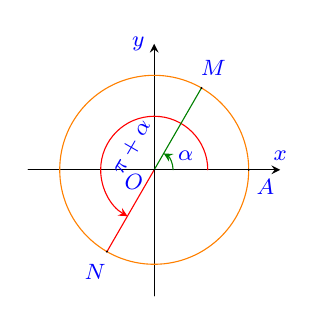
\begin{tikzpicture}[line join = round, line cap = round, >=stealth, font=\footnotesize, scale=0.4]
				\tikzset{label style/.style={font=\footnotesize}}
				\path (0,0) coordinate (O)
				(3,0) coordinate (A)
				(0:0)++(60:3) coordinate (M)
				(0:0)++(240:3) coordinate (N)
				;
				\draw[->] (-4,0) -- (4,0) node[above,blue]{$x$};
				\draw[->] (0,-4) -- (0.,4) node[left,blue]{$y$};
				\draw[orange] (O) circle (3cm);
				\draw[rotate=0,->,red] (1.7,0) arc (0:240:1.7cm);
				\draw[rotate=0,->,green!50!black] (0.6,0) arc (0:60:0.6cm);
				\draw (1,0) node[above,blue] {$\alpha$};
				\draw (-1.2,1) node[below,blue,rotate=60]{$\pi+\alpha$};
				\draw[red] (O)--(N);
				\draw[green!50!black] (O)--(M);
				\foreach \p/\r in {A/-45,M/60,N/240,O/-150}
				\fill (\p) circle (1pt) node[shift={(\r:3mm)},blue]{$\p$};
			\end{tikzpicture}}
	\end{khung4}
\end{multicols}
\newpage

\subsection{Công thức lượng giác}
\subsubsection{Công thức cộng}
\begin{khung4}{Công thức cộng}
	\begin{multicols}{2}
	\begin{itemize}
		\item $\cos (a-b) = \cos a \cos b + \sin a\sin b$.
		\item $\cos (a+b) = \cos a \cos b - \sin a\sin b$.
		\item $\sin (a-b) = \sin a \cos b - \sin b \cos a$.
		\item $\sin (a+b) = \sin a \cos b + \sin b \cos a$.
		\item $\tan (a-b) = \dfrac{\tan a - \tan b}{1+\tan a \tan b}$.
		\item $\tan (a+b) = \dfrac{\tan a + \tan b}{1-\tan a \tan b}$.
	\end{itemize}
\end{multicols}
\end{khung4}
\begin{khung4}{Trường hợp đặc biệt}
	\begin{itemize}
		\item $\sin x + \cos x = \sqrt{2}\sin\left(x+\dfrac{\pi}{4}\right) = \sqrt{2}\cos \left(x-\dfrac{\pi}{4}\right)$.
		\item $\sqrt{3}\sin x + \cos x = 2\sin \left(x+\dfrac{\pi}{6}\right) = 2\cos \left(x-\dfrac{\pi}{3}\right)$.
		\item $\sin x + \sqrt{3}\cos x = 2\sin \left(x+ \dfrac{\pi}{3}\right) = 2\cos \left(x-\dfrac{\pi}{6}\right)$.
	\end{itemize}
\end{khung4}
\subsubsection{Công thức nhân đôi}
\begin{multicols}{2}
	\begin{khung4}{Công thức nhân đôi}
		\begin{itemize}
			\item $\sin 2a = 2\sin a \cos a$.
			\item $\cos 2a = \cos^2a-\sin^2a = 2\cos^2a-1 = 1-2\sin^2a$.
			\item $\tan 2a = \dfrac{2\tan a}{1-\tan^2a}$.
		\end{itemize}
	\end{khung4}
	\begin{khung4}{Công thức hạ bậc}
		\begin{itemize}
			\item $\sin^2a= \dfrac{1-\cos 2a}{2}$.
			\item $\cos^2a = \dfrac{1+\cos 2a}{2}$.
			\item $\tan^2a=\dfrac{1-\cos2a}{1+\cos 2a}$.
		\end{itemize}
	\end{khung4}
\end{multicols}

\begin{note}
	Áp dụng công thức cộng cho $3a = a +2a$, ta có công thức nhân ba:
\end{note}
\begin{khung4}{Công thức nhân ba}
	\begin{multicols}{2}
	\begin{itemize}
		\item $\sin3a= 3\sin a -4\sin^3a$.		
		\item $\cos3a= 4\cos^3a-3\cos a$.
		\item $\tan3a = \dfrac{3\tan a - \tan^3 a}{1-3\tan^2a}$.
	\end{itemize}
\end{multicols}
\end{khung4}

\subsubsection{Công thức biến đổi tích thành tổng}
\begin{khung4}{Công thức tích thành tổng}
	\begin{multicols}{2}
	\begin{itemize}
		\item $\cos a \cos b = \dfrac{1}{2}\left[\cos (a-b) + \cos (a+b)\right]$.
		\item $\sin a \sin b = \dfrac{1}{2}\left[\cos (a-b)-\cos(a+b)\right]$.
		\item $\sin a \cos b = \dfrac{1}{2}\left[\sin (a-b)+\sin (a+b)\right]$.
	\end{itemize}
	\end{multicols}
\end{khung4}
\subsubsection{Công thức biến đổi tổng thành tích}
Công thức biến đổi tổng thành tích được xây dựng bằng cách $a=\dfrac{a+b}{2}, b = \dfrac{a-b}{2}$ trong công thức biến đổi tích thành tổng.
\begin{khung4}{Công thức tổng thành tích}
	\begin{multicols}{2}
	\begin{itemize}
		\item $\cos a+ \cos b = 2\cos\dfrac{a+b}{2}\cos \dfrac{a-b}{2}$.
		\item $\cos a- \cos b = -2\sin\dfrac{a+b}{2}\sin \dfrac{a-b}{2}$.
		\item $\sin a+ \sin b = 2\sin\dfrac{a+b}{2}\cos \dfrac{a-b}{2}$.
		\item $\sin a -\sin b = 2\cos\dfrac{a+b}{2}\sin \dfrac{a-b}{2}$.
	\end{itemize}
\end{multicols}
\end{khung4}
\newpage

\subsection{Hàm số lượng giác}
\begin{khung4}{Hàm số chẵn, hàm số lẻ}
	\begin{multicols}{2}
		\begin{itemize}
			\item Hàm số $f(x)$ được gọi là \textbf{hàm số chẵn} nếu $\forall x \in \mathscr{D}$ thì $-x \in \mathscr{D}$ và $f(-x)=f(x)$. Đồ thị của một \textbf{hàm số chẵn} nhận \textbf{trục tung} là trục đối xứng.
			\item Hàm số $f(x)$ được gọi là \textbf{hàm số lẻ} nếu $\forall x \in \mathscr{D}$ thì $-x \in \mathscr{D}$ và $f(-x)=-f(x)$. Đồ thị của một \textbf{hàm số lẻ} nhận \textbf{gốc toạ độ} là tâm đối xứng.
		\end{itemize}
	\end{multicols}
	Các hàm số $y=\sin x$, $y=\tan x$, $y=\cot x$ là hàm số \textit{lẻ}, hàm số $y=\cos x$ là hàm số \textit{chẵn}.
\end{khung4}
\begin{khung4}{Hàm số tuần hoàn}
	\begin{dn}
		Hàm số $y=f(x)$ có tập xác định $\mathscr{D}$ được gọi là \textbf{hàm số tuần hoàn} nếu tồn tại số $T \neq 0$ sao cho với mọi $x \in \mathscr{D}$ ta có:
		\begin{itemize}
			\item $x+T \in \mathscr{D}$ và $x-T \in \mathscr{D}$;
			\item $f(x+T)=f(x)$.
		\end{itemize}
		Số $T$ dương nhỏ nhất thỏa mãn các điều kiện trên (nếu có) được gọi là \textbf{chu kì} của hàm số tuần hoàn đó.
	\end{dn}
	Các hàm số $y=A \sin \omega x$ và $y=A \cos \omega x$ $(\omega>0)$ là những hàm số tuần hoàn với chu kì $T=\dfrac{2 \pi}{\omega}$.\\
	Các hàm số $y=A \tan \omega x$ và $y=A \cot \omega x$ $(\omega>0)$ là những hàm số tuần hoàn với chu kì $T=\dfrac{\pi}{\omega}$.
\end{khung4}
\begin{center}
	\begin{tikzpicture}[line join = round, line cap = round, >=stealth, font=\small, thick, scale=.7]
		\path (0,0) coordinate (O)
		(3,0) coordinate (A)
		(0,3) coordinate (B)
		(0,-3) coordinate (B')
		(-3,0) coordinate (A');
		\draw[->] (-4,0) -- (4,0) node[above,blue]{$\cos$};
		\draw[->] (0,-4) -- (0.,3.5) node[left,blue]{$\sin$};
		\draw[orange] (O) circle (3cm);
		\draw[->,green!50!black] (40:3.5) arc (40:50:3.5cm) node[midway,above right] {(+)};
		\draw[->,green!50!black](5,0)node[align=center,rotate=90,below]{$\sin x$ đồng biến\\ trên $\left(-\dfrac{\pi}{2}+k2\pi;\dfrac{\pi}{2}+k2\pi\right)$}
		(-30:5) arc (-30:30:5cm) ;
		\draw[->,red!50!black](0,5)node[align=center,above]{$\cos x$ nghịch biến\\ trên $\left(k2\pi;\pi+k2\pi\right)$}
		(60:5) arc (60:120:5cm) ;
		\draw[->,red!50!black](-5,0)node[align=center,rotate=-90,below]{$\sin x$ nghịch biến\\ trên $\left(\dfrac{\pi}{2}+k2\pi;\dfrac{3\pi}{2}+k2\pi\right)$}
		(150:5) arc (150:210:5cm) ;

		\draw[->,green!50!black](0,-5)node[align=center,below]{$\cos x$ đồng biến\\ trên $\left(-\pi+k2\pi;k2\pi\right)$}
		(-120:5) arc (-120:-60:5cm) ;

		\foreach \p/\r in {A/-45,O/-150,A'/-135,B'/-45,B/45}
		\fill (\p) circle (1pt) node[shift={(\r:3mm)},blue]{$\p$};
	\end{tikzpicture}
\end{center}

\subsection{Phương trình lượng giác}
\begin{khung4}{Phương trình $\sin x = a$.}
	\begin{enumerate}[\faCheckSquareO]
		\item Trường hợp $a>1$ hoặc $a<-1$ phương trình vô nghiệm.
		\item Trường hợp $a \in \{-1;0;1\}$.
		      \begin{multicols}{3}
			      \begin{tikzpicture}[smooth,samples=300,scale=0.8,>=stealth]
				      \draw[->] (-1.5,0)--(1.5,0) node[below]{\footnotesize$cos$};
				      \draw[->] (0,-1.5)--(0,1.8) node[right]{\footnotesize$sin$};
				      \draw (0,0) node[below left]{\footnotesize$O$};
				      \tkzDefPoints{0/0/I}
				      \draw[orange] (I) circle(1cm);
				      \draw[fill,blue] (0,1) circle(2.5pt) node[above left] {$B$};
				      \node[below] at (0,-1.5) {\fbox{$\sin x=1 \Leftrightarrow x=\tfrac{\pi}{2}+k2\pi$}};
			      \end{tikzpicture}
			      \hspace{-0.4cm}
			      \begin{tikzpicture}[smooth,samples=300,scale=0.8,>=stealth]
				      \draw[->] (-1.5,0)--(1.5,0) node[below]{\footnotesize$cos$};
				      \draw[->] (0,-1.5)--(0,1.8) node[right]{\footnotesize$sin$};
				      \draw (0,0) node[below left]{\footnotesize$O$};
				      \tkzDefPoints{0/0/I}
				      \draw[orange] (I) circle(1cm);
				      \draw[fill,blue] (0,-1) circle(2.5pt)node[below left] {$B'$};
				      \node[below] at (0,-1.5) {\fbox{$\sin x=-1 \Leftrightarrow x=-\tfrac{\pi}{2}+k2\pi$}};
			      \end{tikzpicture}
			      \hspace{-0.4cm}
			      \begin{tikzpicture}[smooth,samples=300,scale=0.8,>=stealth]
				      \draw[->] (-1.5,0)--(1.5,0) node[below]{\footnotesize$cos$};
				      \draw[->] (0,-1.5)--(0,1.8) node[right]{\footnotesize$sin$};
				      \draw (0,0) node[below left]{\footnotesize$O$};
				      \tkzDefPoints{0/0/I}
				      \draw[orange] (I) circle(1cm);
				      \draw[fill,blue] (1,0) circle(2.5pt) (-1,0) circle(2.5pt) node[above right] at (1,0) {$A$};
				      \node[above left,blue] at (-1,0) {$A'$};
				      \node[below] at (0,-1.5) {\fbox{$\sin x=0 \Leftrightarrow x=k\pi$}};
			      \end{tikzpicture}
		      \end{multicols}
		\item Trường hợp $a \in \left\{\pm \dfrac{1}{2};\pm \dfrac{\sqrt{2}}{2};\pm \dfrac{\sqrt{3}}{2}\right\}$ hoặc $a \in (-1;1)$. Ta bấm máy \shiftk \sink để đổi tìm góc $\alpha$ hoặc $\beta^\circ$.
			      \immini{
				      \begin{listEX}[1]
					      \item [\ding{172}] Công thức theo đơn vị rad:
					      $\sin x = \sin \alpha \Leftrightarrow \hoac{&x=\alpha+k2\pi\\&x=\pi-\alpha+k2\pi}, \,k \in \mathbb{Z}$
					      \item [\ding{173}] Công thức theo đơn vị độ: $\sin x = \sin \beta^\circ \Leftrightarrow \hoac{&x=\beta^\circ+k360^\circ\\&x=180^\circ-\beta^\circ+k360^\circ}, \,k \in \mathbb{Z}$
				      \end{listEX}
			      }{\begin{tikzpicture}[smooth,samples=300,scale=1,>=stealth]
					      \draw[->] (-1.5,0)--(1.5,0);
					      \draw[->] (0,-1.3)--(0,1.5) node[right]{\footnotesize$sin$};
					      \draw (0,0) node[below left]{\footnotesize$O$};
					      \tkzDefPoints{0/0/I}
					      \draw[orange] (I) circle(1cm);
					      \coordinate (M) at ($(I)+(50:1cm)$);
					      \coordinate (N) at ($(I)+(130:1cm)$);
					      \tkzDrawPoints[size=3,fill=blue](M,N)
					      \tkzDrawSegments(I,M I,N)
					      \tkzDrawSegments[dashed](M,N)
					      \tkzLabelPoints[right,blue](M)
					      \tkzLabelPoints[left,blue](N)
					      \node[below right] at (0,0.7) {$a$};
				      \end{tikzpicture}
			      }
	\end{enumerate}
\end{khung4}
\begin{khung4}{Phương trình $\cos x = a$.}
\begin{enumerate}[\faCheckSquareO]
	\item Trường hợp $a>1$ hoặc $a<-1$ phương trình vô nghiệm.
	\item Trường hợp $a \in \{-1;0;1\}$.
	      \begin{multicols}{3}
		      \begin{tikzpicture}[smooth,samples=300,scale=0.8,>=stealth]
			      \draw[->] (-1.5,0)--(1.8,0) node[below]{\footnotesize$cos$};
			      \draw[->] (0,-1.5)--(0,1.8) node[right]{\footnotesize$sin$};
			      \draw (0,0) node[below left]{\footnotesize$O$};
			      \tkzDefPoints{0/0/I}
			      \draw[orange] (I) circle(1cm);
			      \draw[fill,blue] (1,0) circle(2.5pt)node[above right]  {$A$};
			      \node[below] at (0,-1.5) {\fbox{$\cos x=1 \Leftrightarrow x=k2\pi$}};
		      \end{tikzpicture}
		      \begin{tikzpicture}[smooth,samples=300,scale=0.8,>=stealth]
			      \draw[->] (-1.5,0)--(1.5,0) node[below]{\footnotesize$cos$};
			      \draw[->] (0,-1.8)--(0,1.5) node[right]{\footnotesize$sin$};
			      \draw (0,0) node[below left]{\footnotesize$O$};
			      \tkzDefPoints{0/0/I}
			      \draw[orange] (I) circle(1cm);
			      \draw[fill,blue] (-1,0) circle(2.5pt)node[below left] {$A'$};
			      \node[below] at (0,-1.5) {\fbox{$\cos x=-1 \Leftrightarrow x=\pi+k2\pi$}};
		      \end{tikzpicture}
		      \begin{tikzpicture}[smooth,samples=300,scale=0.8,>=stealth]
			      \draw[->] (-1.5,0)--(1.8,0) node[below]{\footnotesize$cos$};
			      \draw[->] (0,-1.5)--(0,1.5);
			      \draw (0,0) node[below left]{\footnotesize$O$};
			      \tkzDefPoints{0/0/I}
			      \draw[orange] (I) circle(1cm);
			      \draw[fill,blue] (0,1) circle(2.5pt) (0,-1) circle(2.5pt) node[above right] at (0,1) {$B$};
			      \node[below left,blue] at (0,-1) {$B'$};
			      \node[below] at (0,-1.5) {\fbox{$\cos x=0 \Leftrightarrow x=\frac{\pi}{2}+k\pi$}};
		      \end{tikzpicture}
	      \end{multicols}
	\item Trường hợp $a \in \left\{\pm \dfrac{1}{2};\pm \dfrac{\sqrt{2}}{2};\pm \dfrac{\sqrt{3}}{2}\right\}$ hoặc $a \in (-1;1)$. Ta bấm máy \shiftk \cosk để tìm góc $\alpha$ hoặc $\beta^\circ$ tương ứng.
	      \immini{
		      \begin{listEX}[1]
			      \item [\ding{172}] Công thức theo đơn vị rad:
			      $\cos x = \cos \alpha \Leftrightarrow \hoac{&x=\alpha+k2\pi\\&x=-\alpha+k2\pi}, \,k \in \mathbb{Z}$
			      \item [\ding{173}] Công thức theo đơn vị độ: $\cos x = \cos \beta^\circ \Leftrightarrow \hoac{&x=\beta^\circ+k360^\circ\\&x=-\beta^\circ+k360^\circ}, \,k \in \mathbb{Z}$
		      \end{listEX}
	      }{\begin{tikzpicture}[smooth,samples=300,scale=1,>=stealth]
			      \draw[->] (-1.5,0)--(1.7,0)node[above]{\footnotesize$cos$};
			      \draw[->] (0,-1.3)--(0,1.5);
			      \draw (0,0) node[below left]{\footnotesize$O$};
			      \tkzDefPoints{0/0/I}
			      \draw[orange] (I) circle(1cm);
			      \coordinate (M) at ($(I)+(50:1cm)$);
			      \coordinate (N) at ($(I)+(-50:1cm)$);
			      \tkzDrawPoints[size=3,fill=blue](M,N)
			      \tkzDrawSegments(I,M I,N)
			      \tkzDrawSegments[dashed](M,N)
			      \tkzLabelPoints[above,blue](M)
			      \tkzLabelPoints[below,blue](N)
			      \node[below right] at (0.7,0) {$a$};
		      \end{tikzpicture}}
\end{enumerate}
\end{khung4}
\begin{khung4}{Phương trình $\tan x = a$ và $\cot x = b$.}
\begin{enumerate}[\faCheckSquareO]
	\item Trường hợp $a \in \left\{0;\pm \dfrac{\sqrt{3}}{3};\pm 1; \pm \sqrt{3}\right\}$ hoặc $a$ bất kì. Ta bấm máy \shiftk \tank để tìm góc $\alpha$ hoặc $\beta^\circ$ tương ứng.
		      \immini{
			      \begin{listEX}[1]
				      \item [\ding{172}] Công thức theo đơn vị rad:
				      $$\tan x = \tan \alpha \Leftrightarrow x=\alpha+k\pi, \,k \in \mathbb{Z}$$
				      \item [\ding{173}] Công thức theo đơn vị độ:
				      $$\tan x = \tan \beta^\circ \Leftrightarrow x=\beta^\circ +k180^\circ, \,k \in \mathbb{Z}$$
			      \end{listEX}
		      }{\begin{tikzpicture}[smooth,samples=300,scale=1,>=stealth]
				      \draw[->] (-1.5,0)--(1.5,0);
				      \draw[->] (0,-1.3)--(0,1.5);
				      \draw (0,0) node[below right]{\footnotesize$O$};
				      \tkzDefPoints{0/0/I, 1/0.9/A}
				      \draw[orange] (I) circle(1cm);
				      \draw[->] (1,-1.3)--(1,1.5)node[right]{\footnotesize$tan$};
				      \tkzInterLC[R](I,A)(I,1cm)\tkzGetPoints{M}{N}
				      \tkzDrawPoints[size=3,fill=blue](I,M,N,A)
				      \tkzDrawSegments(A,N)
				      \tkzLabelPoints[below,font=\footnotesize,blue](M)
				      \tkzLabelPoints[above,font=\footnotesize,blue](N)
				      \node[right] at (1,0.9) {$a$};
			      \end{tikzpicture}}
\end{enumerate}

\textbf{$\bigstar$ Phương trình $\cot x = b$.}
	$b \in \left\{\pm \dfrac{\sqrt{3}}{3};\pm 1; \pm \sqrt{3}\right\}$ hoặc $b$ bất kì. Ta bấm máy \shiftk \tank \fbox{$\tfrac{1}{b}$} để tìm góc $\alpha$ hoặc $\beta^\circ$ tương ứng. Riêng $b=0$ thì $\alpha=\dfrac{\pi}{2}$. Công thức nghiệm tương tự phương trình $\tan x =a$
\end{khung4}